\section{Example of AlgoView system operation}

Let's look at an example of how the system works using a simple algorithm: “Finding the sum of array elements by doubling.” The doubling method is used as a fast option for computing long sequences of associative operations. Elements at each stage of the algorithm are divided into pairs. Each pair contains the sum of its constituent elements. At the next stage, these sums are divided into pairs, etc. Characteristics of the algorithm (for summing an array of order n): total number of vertices: $n - 1$; critical path length: $\left\lceil{\log_2n}\right\rceil$; canonical width of the parallel form: $n$.

\textbf{Sequential complexity of the algorithm.} To calculate the sum of an array consisting of $n$ elements, for any decomposition of $n$ into pairs, the essence of the algorithm comes down to a simple rearrangement of parentheses in the summation formula. The number of operations is constant and equal to $n-1$. A sequential algorithm should be classified as a \textit{linear complexity} algorithm based on the number of sequential operations.

\textbf{Algorithm parallelism resource.} To sum an array of order $n$ using the doubling method in the parallel version, it is necessary to sequentially execute $\left\lceil{\log_2n}\right\rceil$ tiers with decreasing ones (from $n/2$ to 1) number of summation operations. When classifying by the height of the parallel form, the doubling method therefore refers to algorithms with \textit{logarithmic complexity}. When classified by the width of the parallel form, its complexity will be \textit{linear}.


\begin{figure}
% \vspace{-0.5cm}
\centering
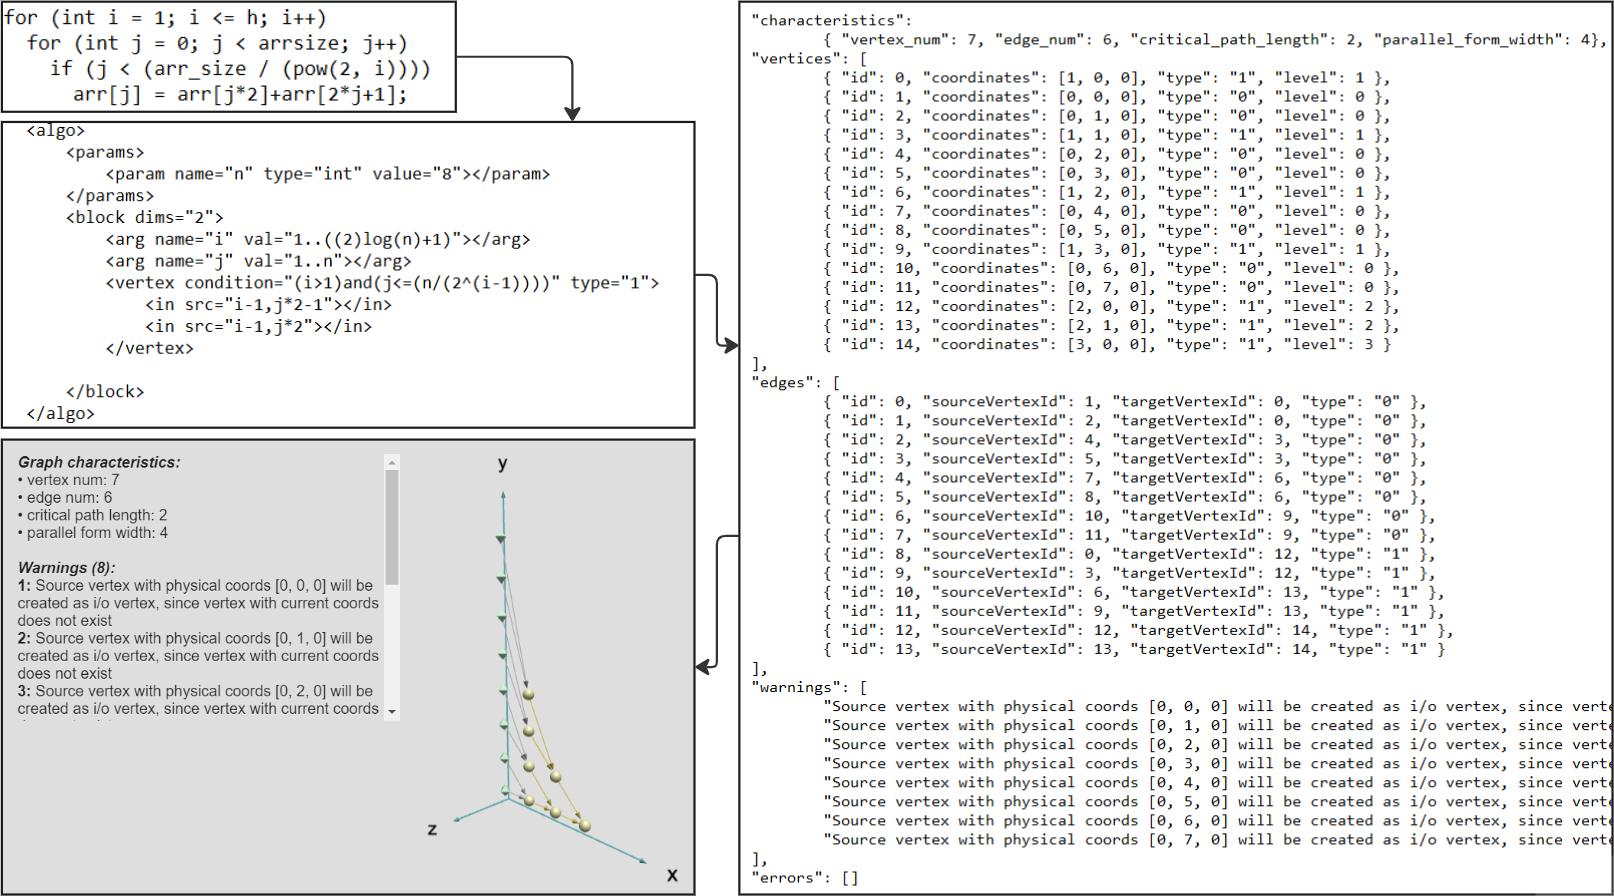
\includegraphics[height=6.78cm]{assets/algo_example.png}
\caption{Operation of the AlgoView system using the example of the algorithm “Finding the sum of array elements by doubling” for $n = 8$ from the implementation of the algorithm in the C language to the final visualization.}
\end{figure}